\documentclass[a3paper,14pt]{extarticle}
\usepackage{extsizes}
\usepackage{cmap}
\usepackage[utf8]{inputenc}
\usepackage[T2A]{fontenc}
\usepackage[english,russian]{babel} 
\usepackage[left=15mm, top=25mm, right=15mm, bottom=30mm, nohead, nofoot]{geometry}
\usepackage{graphicx}  % изобржаения
\usepackage{float} % плавающие объекты
\usepackage{wrapfig}  % изобржаения
\usepackage{tikz} % графика
\usepackage{xcolor} % определение цветов
\usepackage{nicefrac} % красивые дроби
\usepackage{cancel} % сокращение
\usepackage{amsmath,amsfonts,amssymb} % математический пакет
\usepackage{hyperref}  % гиперссылки
\usepackage{fancybox,fancyhdr} % хедер и футер
\pagestyle{fancy}
\fancyhf{}
\fancyhead[L]{Практическая линейная алгебра}
\fancyhead[R]{Овчинников Павел}
\fancyfoot[C]{\thepage}
\setcounter{page}{1}
\headsep=10mm
\footskip=15mm

\definecolor{urlcolor}{HTML}{3454D1}
\definecolor{linkcolor}{HTML}{3454D1}
\hypersetup{pdfstartview=FitH, linkcolor=linkcolor, urlcolor=urlcolor, colorlinks=true}

\newlength{\tempheight}
\newcommand{\Let}{
\mathbin{\text{\settoheight{\tempheight}{\mathstrut}\raisebox{0.4\pgflinewidth}{
\tikz[baseline=0.5ex,line cap=round,line join=round] \draw (0,0) --++ (0.3em,0) --++ (0,2.3ex) --++ (-0.3em,0);
}}}}
\newcommand*\circled[1]{\tikz[baseline=(char.base)]{
            \node[shape=circle,draw,inner sep=2pt] (char) {#1};}}
\newcommand*\squared[1]{\tikz[baseline=(char.base)]{
            \node[shape=rectangle,draw,inner sep=4pt] (char) {$#1$};}}
\newcommand{\at}{\biggr\rvert}
\newcommand{\shiftright}[3]{\makebox[#2][r]{\makebox[#1][l]{#3}}}

\newcommand\NB{\textbf{N\kern-0.32em\textcolor{red}{B}}}
\newcommand{\observ}[1]{\textbf{\textit{Рубрика «наблюдения»}:} \textit{#1}}

\begin{document}
\section*{\centering Лабораторная работа №6}
\subsection*{\centering Задание №1. Как зовут жирафа, который занимается линейной алгеброй? \\ Sильвестр Vладимирович Dжирафский!}
Привет! Время выбрать весёлую картинку, чтобы мощно сжать её\dots\ Выбор широкий, но мы то знаем, как получить зачёт автоматом ;)
\begin{figure}[H]
    \centering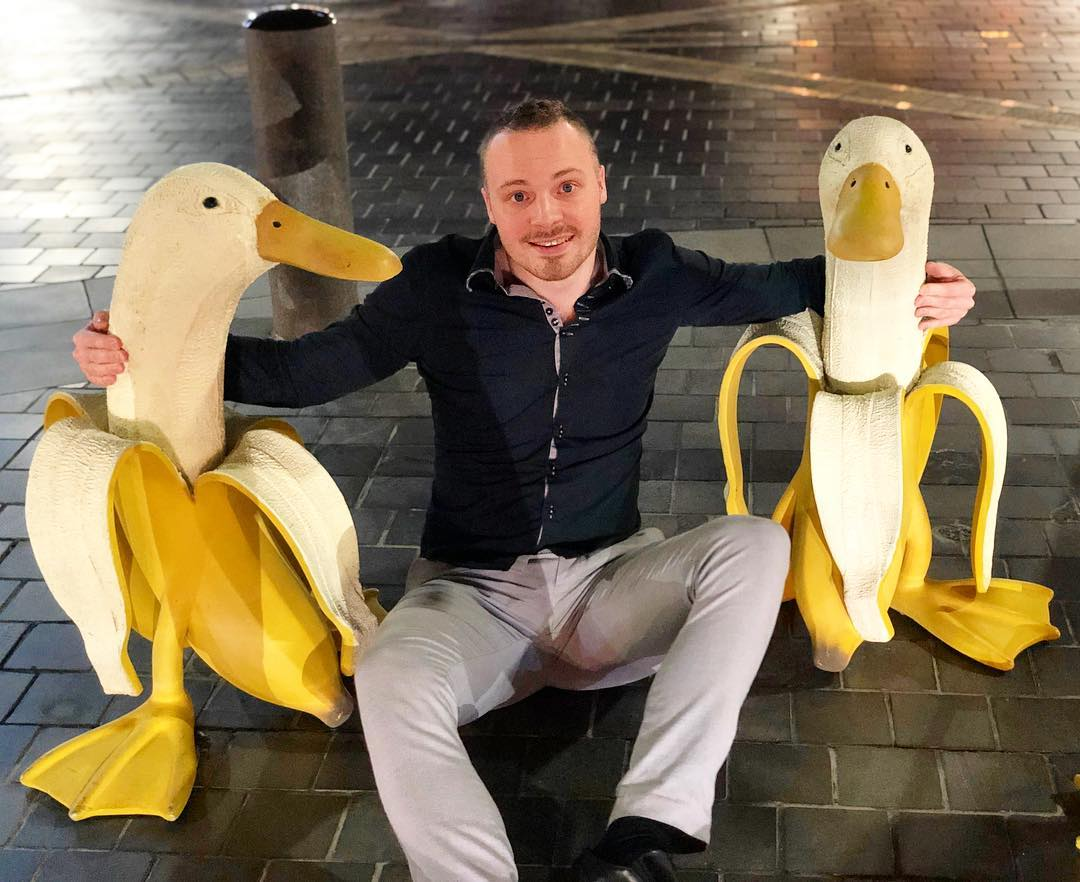
\includegraphics[width=0.4\textwidth]{banana ducks.jpg}
    \caption{Красавчик с двумя банановыми утками, которого мы сжимаем.}
\end{figure} \noindent
И сегодня именно он станет героем нашей лабораторной работы. Чтобы вся магия сжатия работала, нам придётся сделать всё немного грустным с нотками вьетнамских флешбеков --- то есть чёрно-белым. Но не беда, мы всё равно сделаем это красиво, с помощью Python и модуля \texttt{Pillow}.
\begin{figure}[H]
    \centering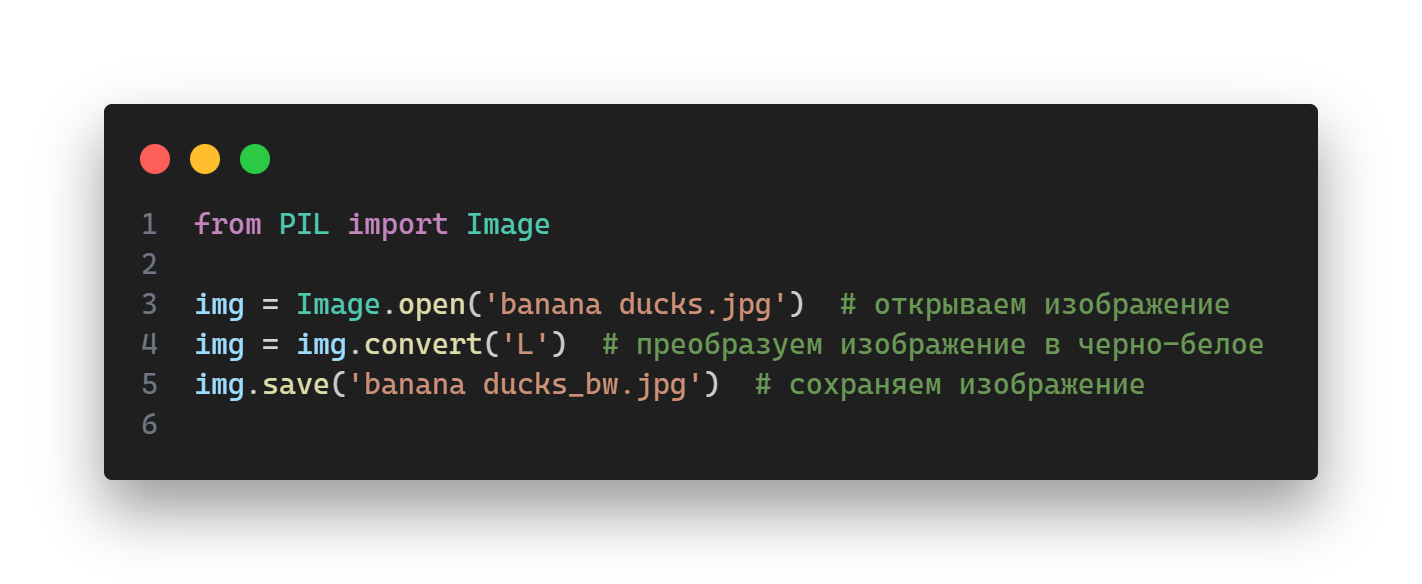
\includegraphics[width=0.58\textwidth]{code1.png}
\end{figure} \noindent
И вот мы получаем вот такое невесёлое изображение:
\begin{figure}[H]
    \centering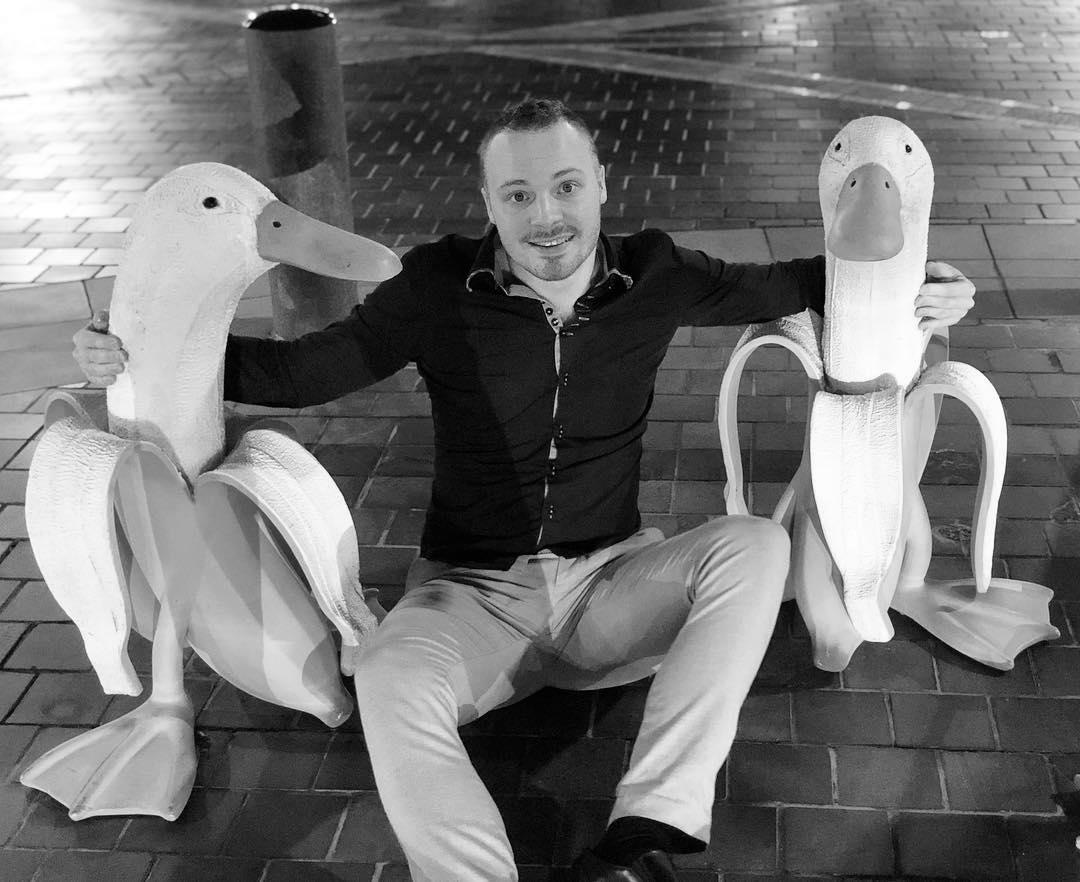
\includegraphics[width=0.4\textwidth]{banana ducks_bw.jpg}
    \caption{В этом красавчике с двумя банановыми утками 952560 чисел.}
\end{figure} \noindent
Ну да, выглядит грустненько, но мы же знаем, что это всего лишь промежуточный этап.

\pagebreak \noindent Теперь нам нужно представить это изображение в виде матрицы и, конечно же, выводить страшный список из 952560 чисел мы абсолютно точно не будем, поэтому выведем матрицу так, как её представляет \texttt{numpy}:
\begin{figure}[H]
    \begin{minipage}{0.63\textwidth}
        \centering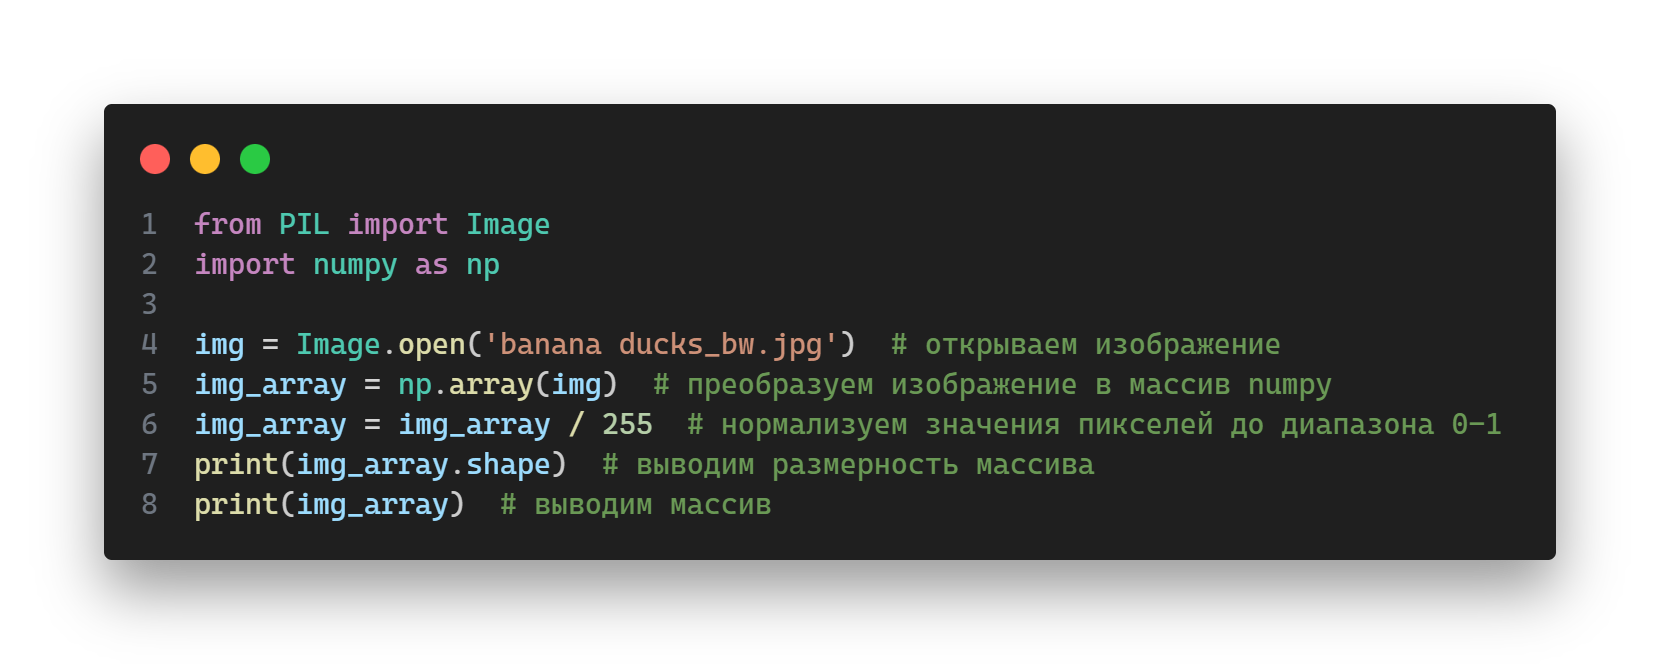
\includegraphics[width=\textwidth]{code2.png}
    \end{minipage}\hfill
    \begin{minipage}{0.33\textwidth}
        \centering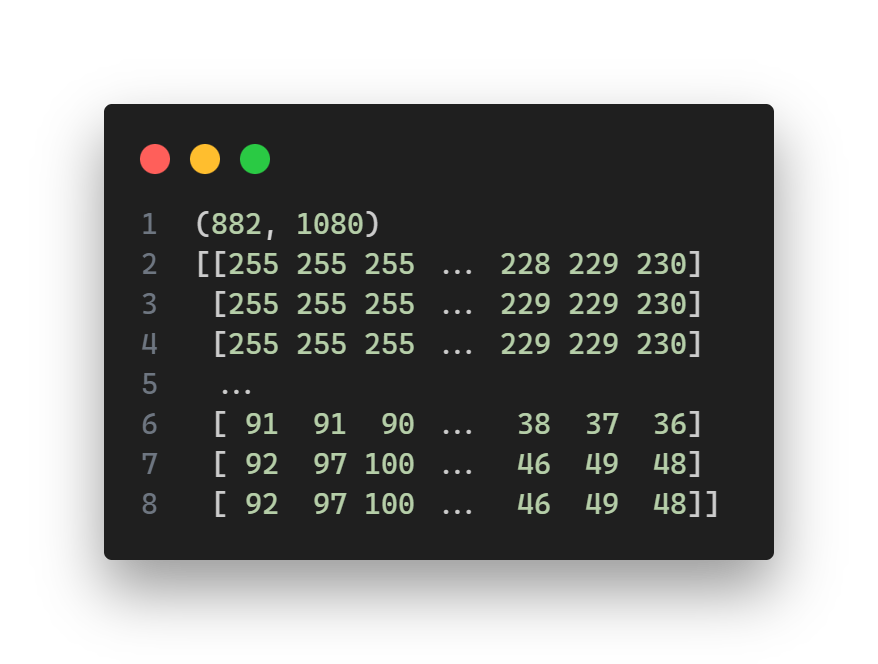
\includegraphics[width=\textwidth]{output1.png}
    \end{minipage}
\end{figure} \noindent
Действительно, в левом верхнем углу белое пятное, справа сверху немного светло, левый нижний край чуть тёмный, а справа снизу совсем темно. Всё верно, всё работает. Теперь мы можем сжать изображение, применив к нему сингулярное разложение. Для этого нам нужно найти это разложение для его матрицы, а потом взять только первые $k$ компонент. И чтобы это сделать, мы воспользуемся функцией \texttt{numpy.linalg.svd}:
\begin{figure}[H]
    \centering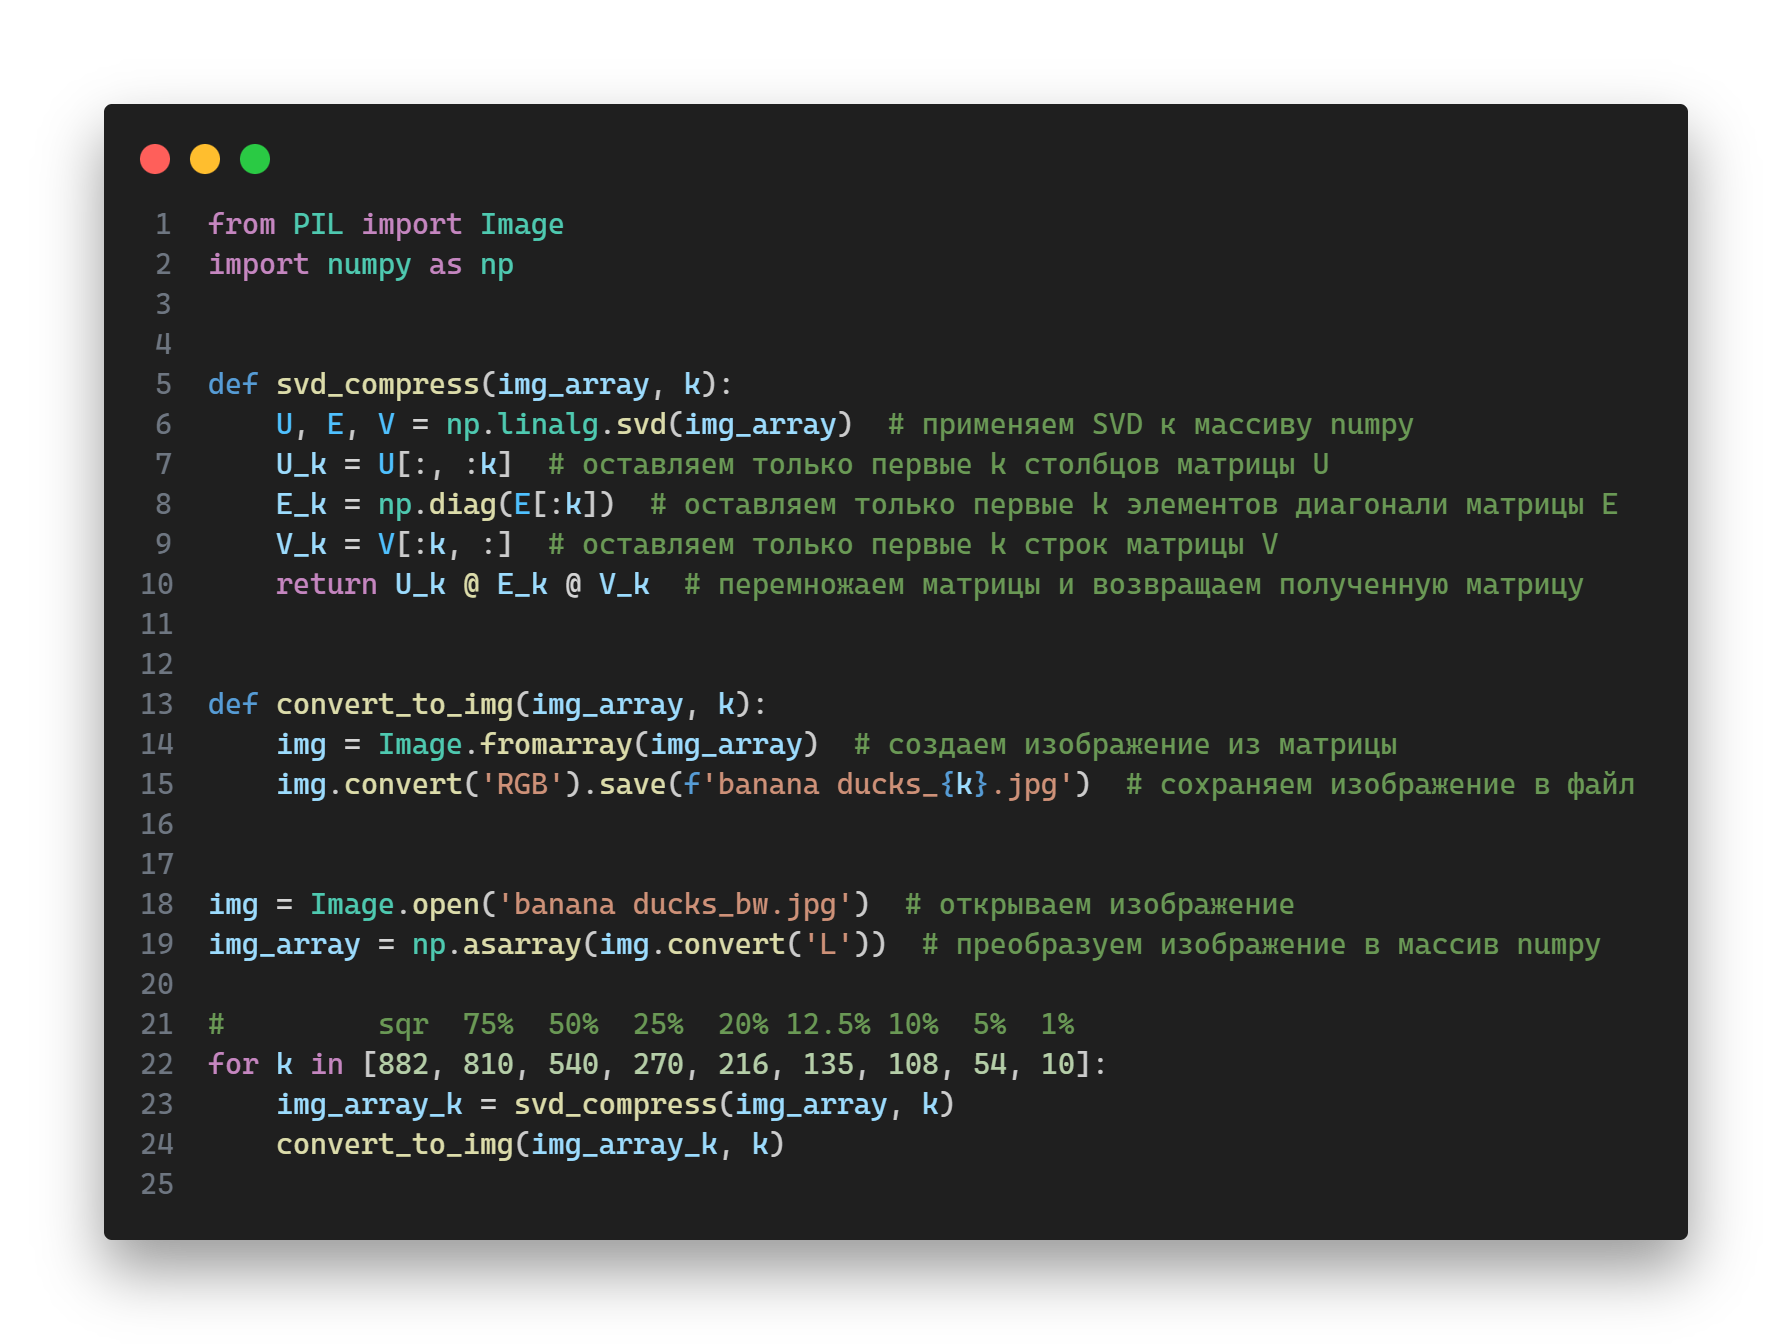
\includegraphics[width=0.8\textwidth]{code3.png}
\end{figure} \noindent
В строках 6-11 описана функция \texttt{svd\_compress}, принимающая на вход матрицу изображения и коэффициент $k$ и возвращающая матрицу, полученную из произведения укороченного SVD. В строках 15-18 описана функция \texttt{convert\_to\_img}, которая принимает на вход матрицу изображения, преобразует её обратно в изображение и сохраняет его в файл. Затем мы открываем наше грустное изображение и балуемся с ним, оставляя в нём всё меньше и меньше сингулярных чисел от матрицы $882\times882$ до $10\times10$.\\[1em]
Для исходного изображения было необходимо хранить в полном SVD $1945206$ чисел, что сильно больше $952560$, однако в reduced-SVD (с отрезанными лишними нулями в матрице $\Sigma$) хранится уже $1731366$ чисел. А можно ли ещё сжать? Конечно! Под каждым из изображений я оставлю подпись, содержающую процент сжатия, выбранное $k$ и количество чисел, необходимое для хранения сжатого изображения. Ну что, поехали!

\begin{figure}[H]
    \begin{minipage}{0.45\textwidth}
        \centering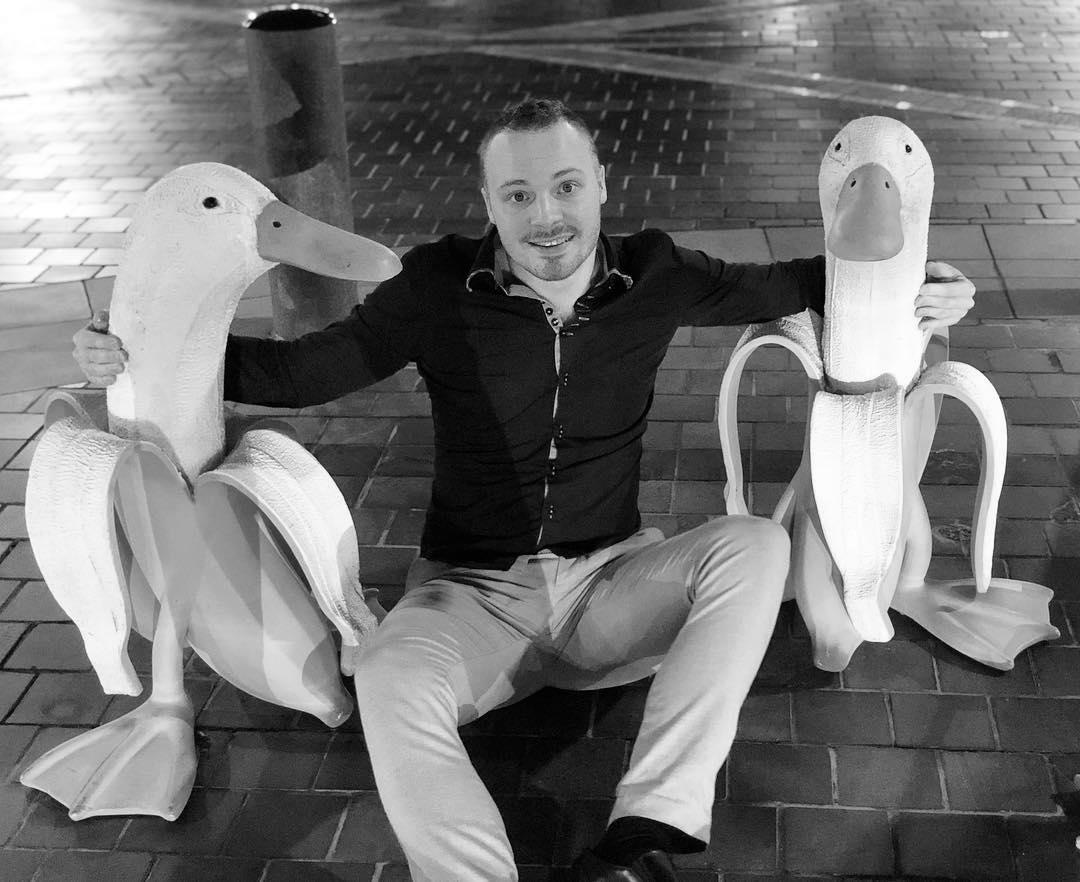
\includegraphics[width=\textwidth]{banana ducks_882.jpg}
        \caption{Сжатие на 18.33\% ($k=882$), 1731366 чисел.\\}
    \end{minipage}\hfill
    \begin{minipage}{0.45\textwidth}
        \centering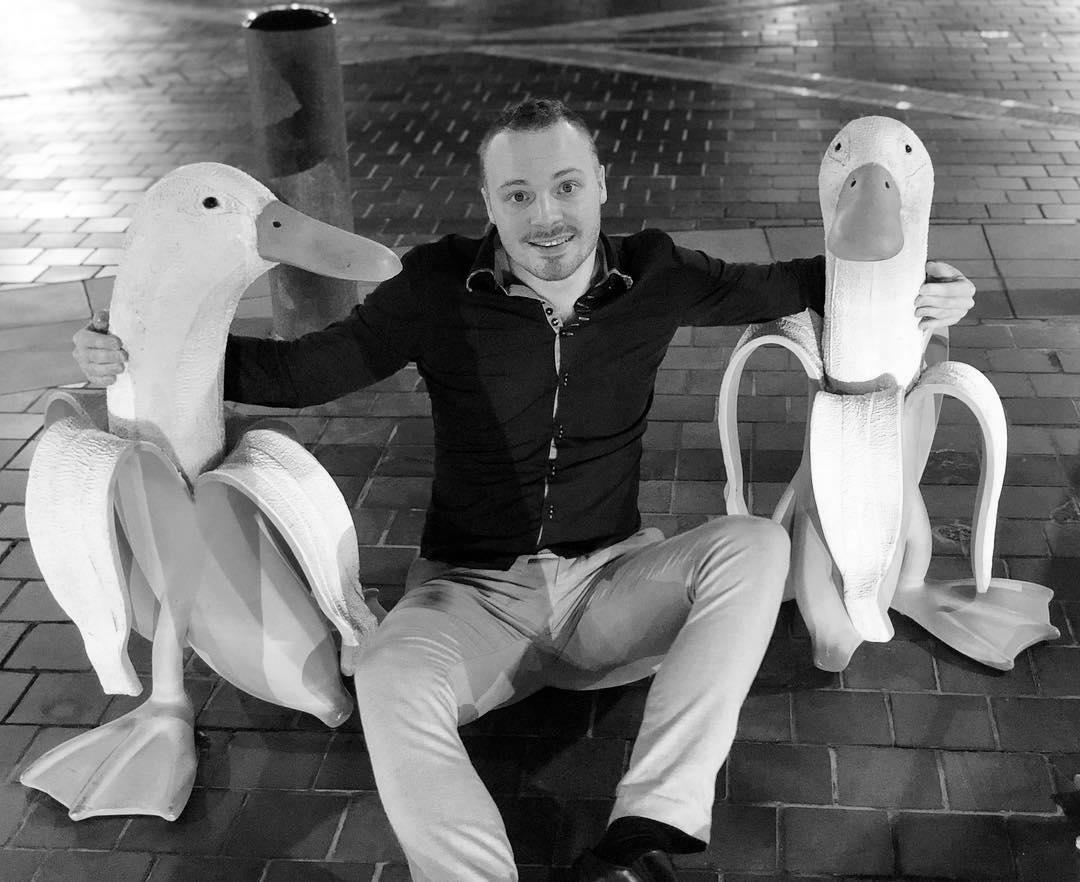
\includegraphics[width=\textwidth]{banana ducks_810.jpg}
        \caption{Сжатие на 25\% ($k=810$), 1590030 чисел.}
    \end{minipage}\\[1em]
    \begin{minipage}{0.45\textwidth}
        \centering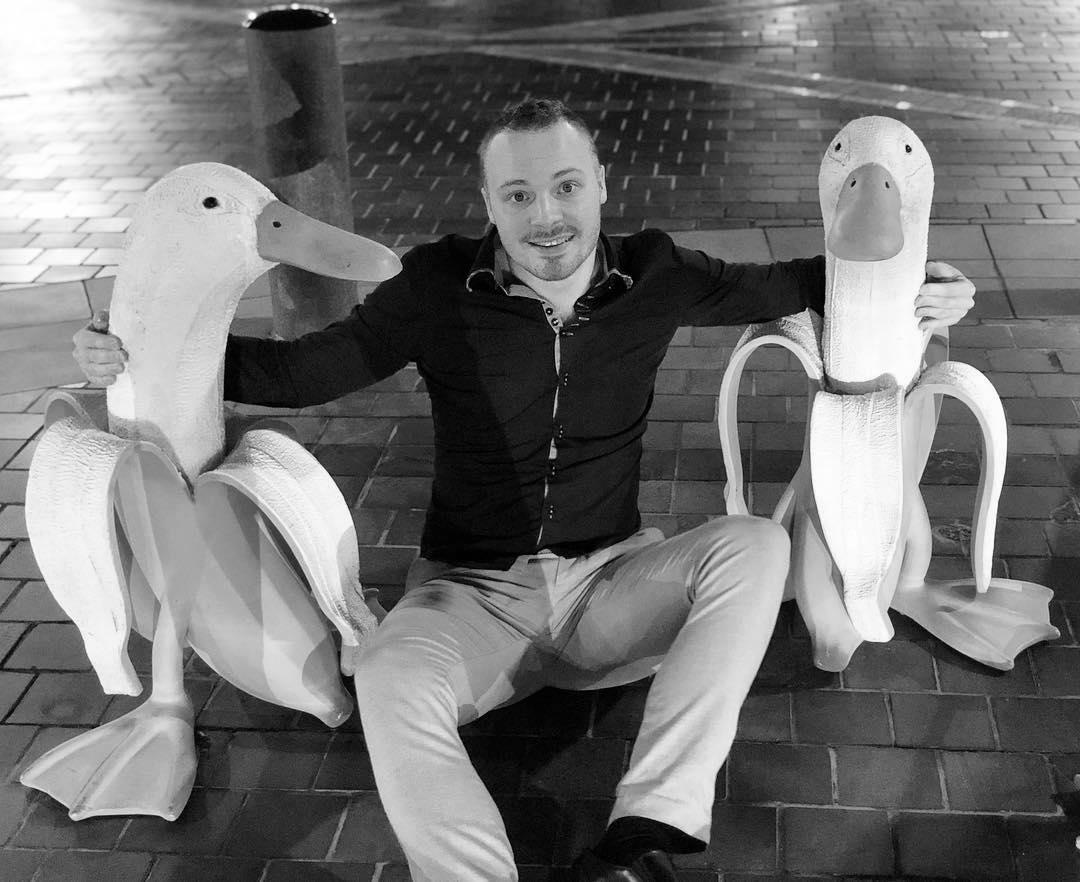
\includegraphics[width=\textwidth]{banana ducks_540.jpg}
        \caption{Сжатие на 50\% ($k=540$), 1060020 чисел.}
    \end{minipage}\hfill
    \begin{minipage}{0.45\textwidth}
        \centering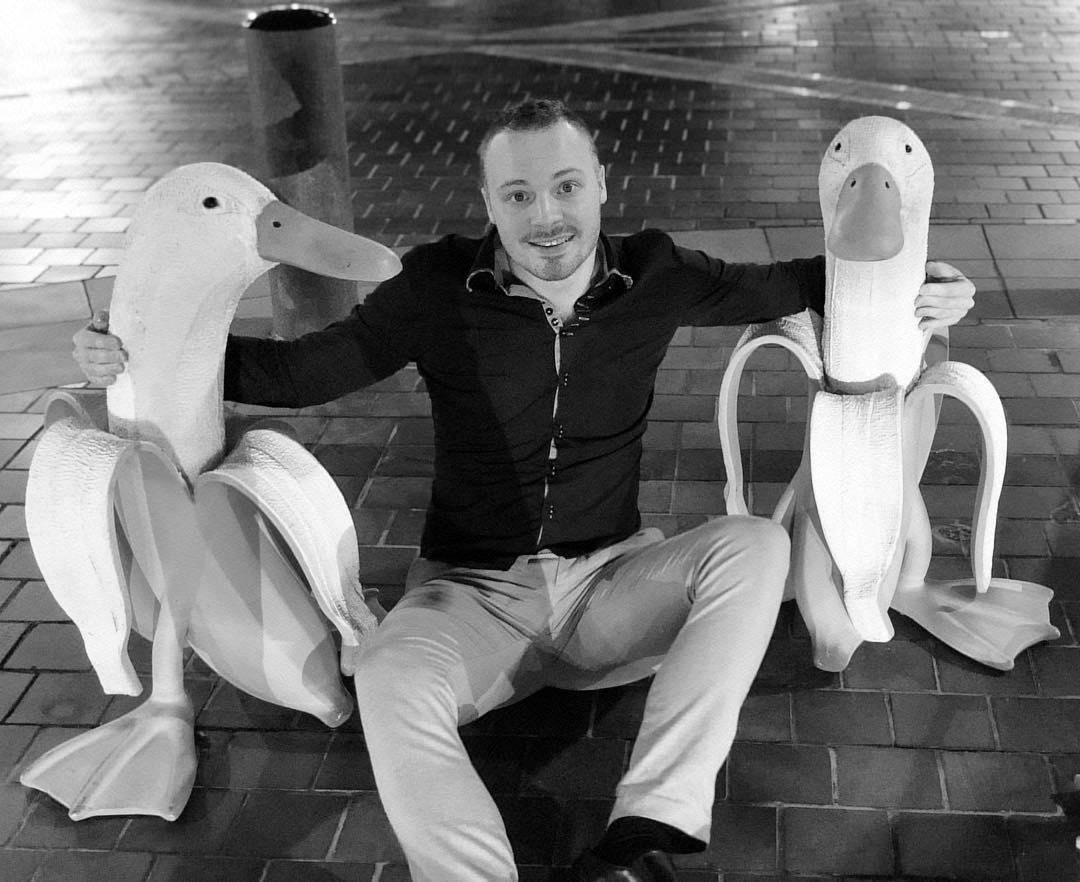
\includegraphics[width=\textwidth]{banana ducks_270.jpg}
        \caption{Сжатие на 75\% ($k=270$), \textbf{530010} чисел.}
    \end{minipage}
\end{figure}
\begin{figure}[H]
    \begin{minipage}{0.45\textwidth}
        \centering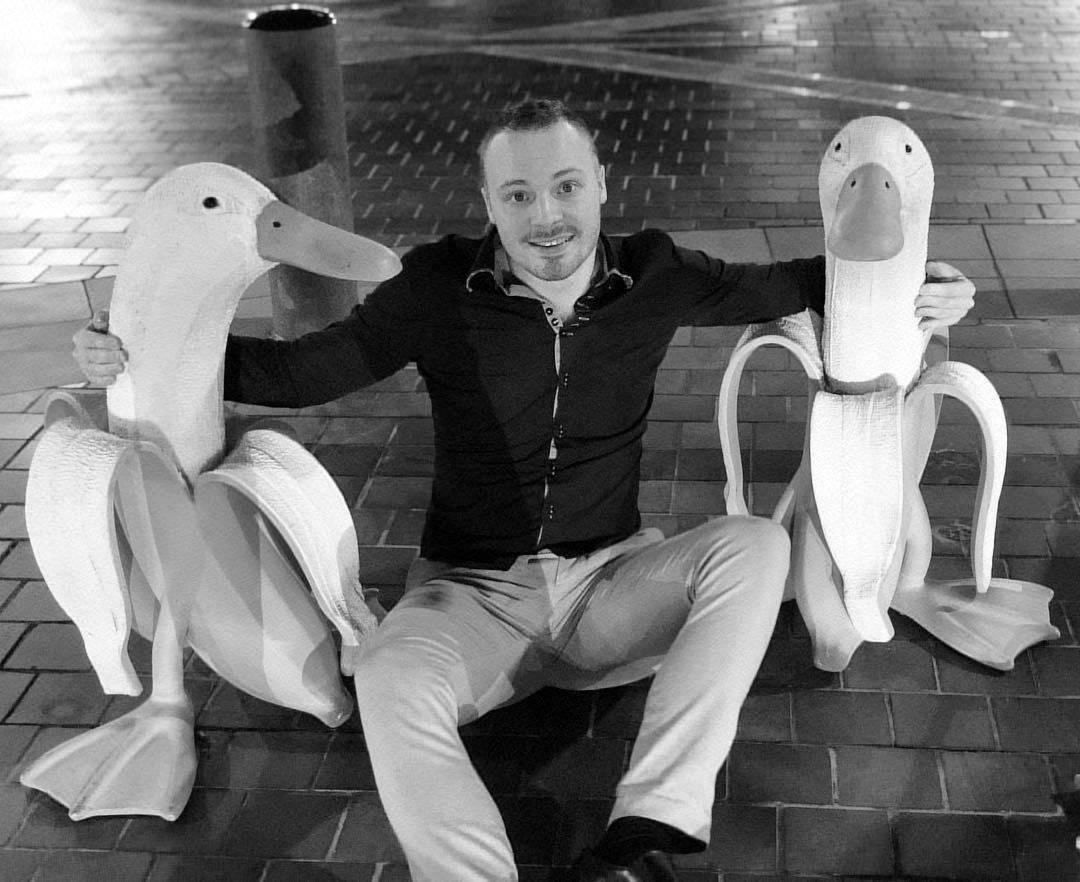
\includegraphics[width=\textwidth]{banana ducks_216.jpg}
        \caption{Сжатие на 80\% ($k=216$), 424008 чисел.}
    \end{minipage}\hfill
    \begin{minipage}{0.45\textwidth}
        \centering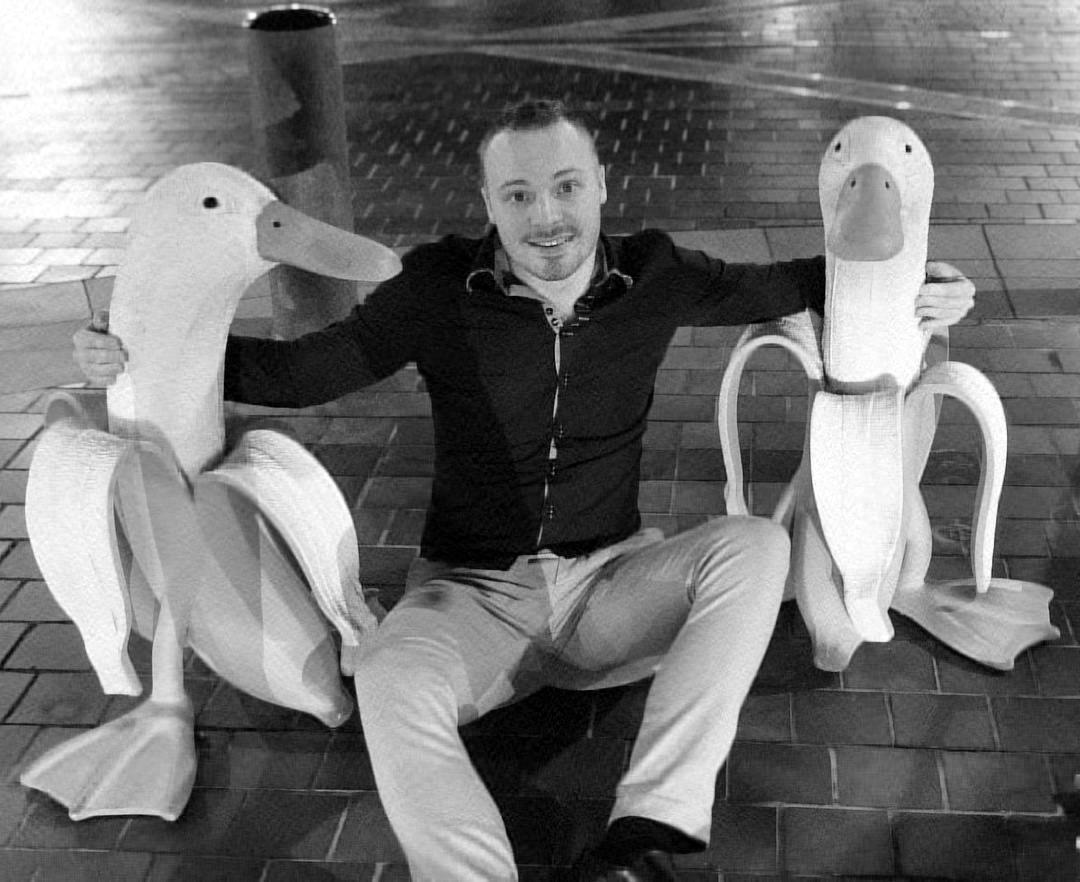
\includegraphics[width=\textwidth]{banana ducks_135.jpg}
        \caption{Сжатие на 87.5\% ($k=135$), 265005 чисел.}
    \end{minipage}
\end{figure}
\begin{figure}[H]
    \begin{minipage}{0.45\textwidth}
        \centering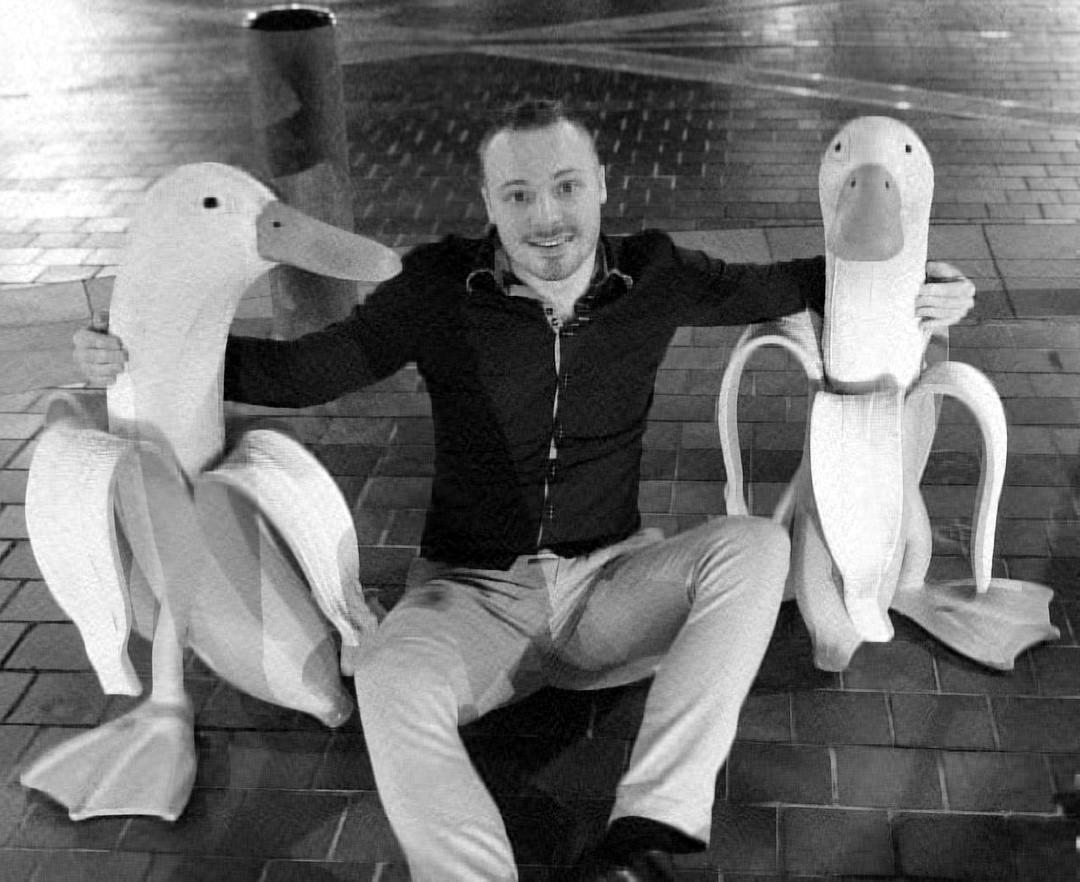
\includegraphics[width=\textwidth]{banana ducks_108.jpg}
        \caption{Сжатие на 90\% ($k=108$), 212004 чисел.}
    \end{minipage}\hfill
    \begin{minipage}{0.45\textwidth}
        \centering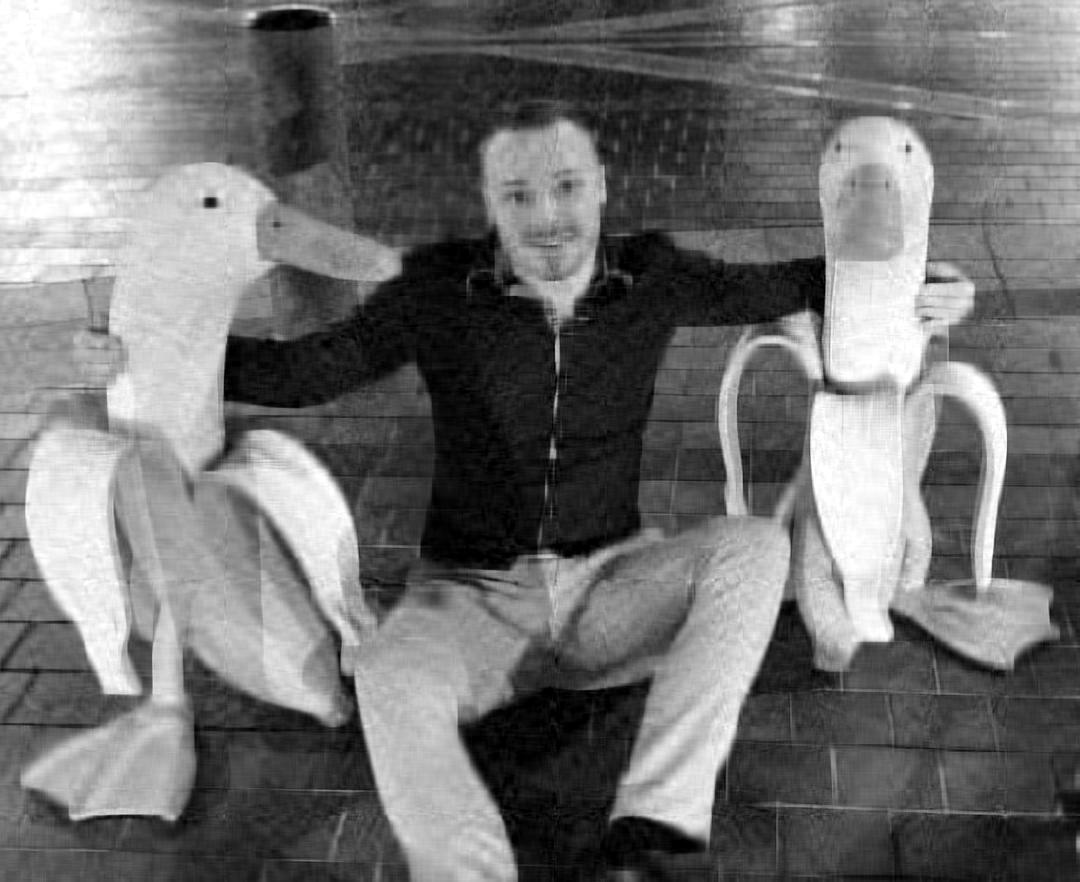
\includegraphics[width=\textwidth]{banana ducks_54.jpg}
        \caption{Сжатие на 95\% ($k=54$), 106002 чисел.}
    \end{minipage}
\end{figure}
\begin{figure}[H]
    \begin{center}
        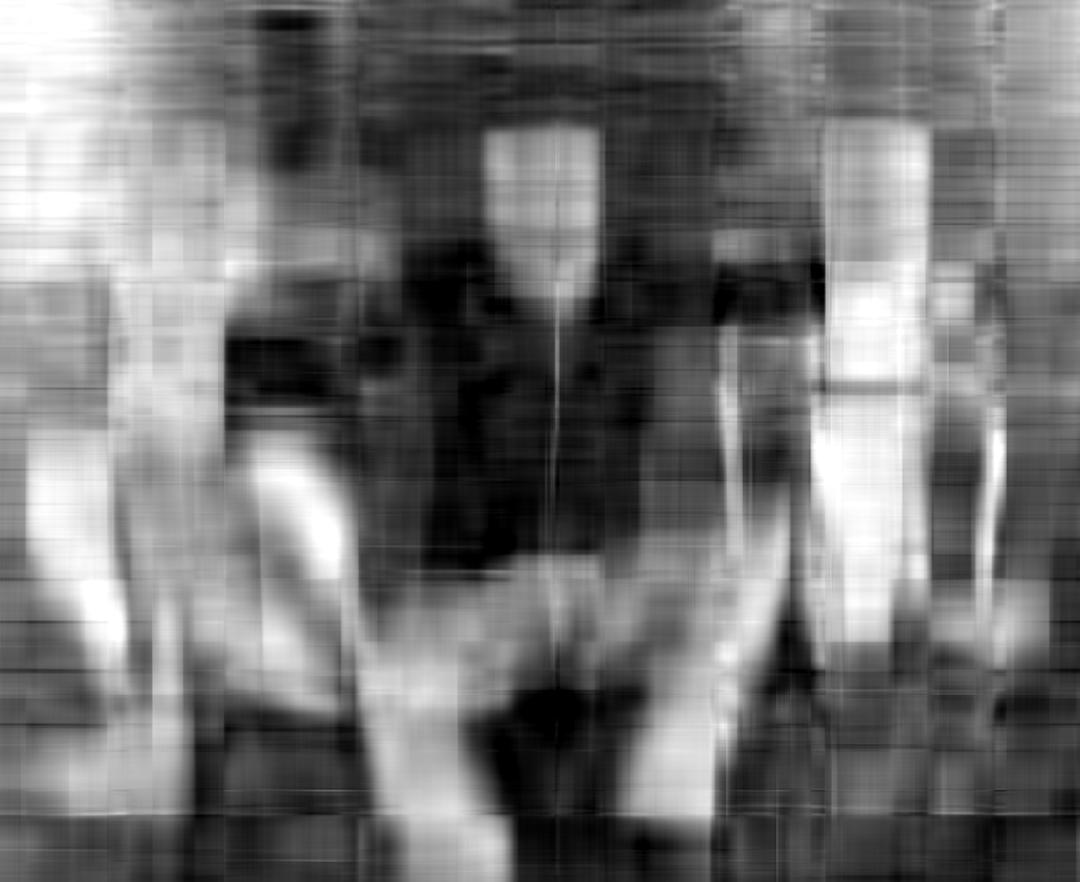
\includegraphics[width=0.45\textwidth]{banana ducks_10.jpg}
        \caption{Сжатие на 99.07\% ($k=10$), 19630 чисел.}
    \end{center}
\end{figure}
\noindent И что же это получается, декомпозиция Перегудина? Оставляю этот вопрос на размышление читателю\dots\ А я пойду поплачу, потому что мне жалко этого красавчика с двумя банановыми утками.
\subsection*{\centering Подводим выводы, делаем итоги}
\begin{itemize}
    \item Чем меньше $k$, тем меньше сингулярных чисел формируют матрицу и тем меньше она похоже на изначальную, но из-за этого больше сжатие, которое ухудшает качество изображения.
    \item Фактически вес файла не изменяется, т.к. JPG и так использует оптимальные технологии сжатия, но если бы мы строили свою технологию сжатия, основанную на сингулярных разложениях, то вес в некоторых случаях можно заметно уменьшить без заметной глазу потери качества.
    \item Эффективными оказались сжатия на $75-87.5\%$. Они требуют для хранения меньше памяти, чем исходная чёрно-белая картинка, но при этом качество изображения остаётся достаточно приемлемым.
    \item Картинка всё ещё различима на сжатиях на $90-95\%$, но качество здесь гораздо хуже.
    \item Картинка полностью неразличима на сжатии на $99.07\%$, но при этом требуется всего $19630$ чисел для хранения, что в $48.5$ раз меньше, чем в исходной картинке.
\end{itemize}

\end{document}